\section{Evaluation}
\label{sec:eval}

We evaluate \sys using four key questions:

\begin{itemize}[leftmargin=*]
  \item \textbf{RQ1 (Single-Tenant Memory/Scheduling):} How much performance gain can \sys's programmable memory and scheduling policies provide on oversubscribed single-tenant workloads?
  \item \textbf{RQ2 (Multi-Tenant Management):} Does \sys's cross-layer policy framework improve tail latency, throughput, and resource fairness compared to user-space and global policies in multi-tenant settings?
  \item \textbf{RQ3 (Programmability \& Mechanism Overhead):} Is \sys sufficiently programmable to support diverse policies, and what is the overhead of its core mechanisms and observability capabilities?
\end{itemize}

\subsection{Methodology and Setup}

We evaluated \sys on two machines. Server~A is a single-socket Intel Core
Ultra~9 285K processor (24 cores) with 128~GB DDR5 RAM and an NVIDIA RTX~5090
GPU. Server~B is a single-socket Intel Xeon~6787P (86~cores, 2.0~GHz, 336~MB
LLC) with 768~GB DDR5 RAM (512~GB CXL module) and an NVIDIA H100 GPU. Unless
otherwise noted, we report results on Server~A and average each metric over
10 trials; when averaging speedups we use geometric means. We compare against
NVIDIA's CUPTI and NVTX-based profiler stack, NVBit gpumemtrace, default UVM
memory management, and the native GPU scheduler without \sys-based policies, as
well as framework-managed offloading where applicable. We use PyTorch (version 2.9.0), vLLM (version 0.11.0), llama.cpp (version 7101), and Faiss (version 1.13.0) for our evaluation.



\subsection{RQ1: Single-Tenant Memory and Scheduling Policies}

We evaluate \sys's memory policy interface on the application workloads introduced in Section~\ref{sec:eval-app-workloads}, focusing on oversubscribed single-tenant setups where memory placement and prefetching dominate performance.

\subsubsection{Microbenchmarks}

\paragraph{Memory Policy Microbenchmarks.}
We evaluate \sys's memory policies on three representative kernels: \texttt{HotSpot} (stencil-like structured access), \texttt{GEMM} (dense matrix multiplication), and \texttt{KMeans} (sparse/irregular access). We configure varying oversubscription ratios (0.6--0.9$\times$ of working set) to stress UVM migration. We compare \sys policies (e.g., Stride Prefetch, LFU Eviction) against the default driver-managed LRU, measuring execution time and fault reduction.

\paragraph{Single-Tenant Block Scheduler.}
We apply a \sys-based block scheduler driven by the GPU-side interface
(Section~\ref{sec:design-sched}) to workloads with significant load imbalance.
Using a cluster-style launch where persistent worker blocks pull work units
via \texttt{should\_try\_steal}, we evaluate on GEMM with variable matrix sizes where static block assignment leads to some blocks being overloaded while others idle.

We compare three scheduling policies: FixedWork (static block assignment), CLC Baseline (cooperative launch control), and TokenBucket (workload-aware). On imbalanced GEMM with variable MxNxK configurations, TokenBucket achieves 51~µs compared to 67~µs for FixedWork, a 24\% improvement.

\subsubsection{Case Studies}

\paragraph{Expert Offloading (llama.cpp GPT-OSS-120B).}
We evaluate \sys on the GPT-OSS-120B MXFP4 MoE model (59~GiB, 116.83B parameters) in \texttt{llama.cpp}, running on RTX 5090 (32GB). The model requires 1.84$\times$ oversubscription, necessitating CPU-GPU memory tiering. We compare five configurations: framework-managed CPU offloading (\texttt{ncmoe=32/64}), default UVM, UVM with user-space hints (\texttt{cudaMemAdvise}), and \sys with eBPF-based expert prefetching.

\Cref{fig:llama-expert-offload} shows prefill (pp512) and decode (tg128) throughput across configurations. The key comparison is between \sys's eBPF-based prefetching and llama.cpp's framework-managed CPU offloading (\texttt{ncmoe=32}), which represents the state-of-the-art for this workload:

\begin{itemize}[leftmargin=*]
  \item \textbf{Decode (memory-bound):} \sys achieves 86.89~t/s, \textbf{4.8$\times$ faster} than framework offloading (18.18~t/s with ncmoe=32). The eBPF policy predicts expert activation patterns and prefetches weights before GPU access, effectively hiding PCIe transfer latency. In contrast, framework offloading incurs per-token CPU-GPU transfer overhead during autoregressive decoding.
  \item \textbf{Prefill (compute-bound):} Framework offloading achieves slightly higher throughput (260.14~t/s vs 229.67~t/s, +13\%) by explicitly managing expert placement and avoiding UVM page faults. However, \sys's 12\% prefill overhead is acceptable given the 4.8$\times$ decode improvement---decode dominates end-to-end latency in interactive serving.
  \item \textbf{User hints degrade performance:} Naive \texttt{cudaMemAdviseSetPreferredLocation} causes 39.6\% prefill regression due to eager migration overhead, demonstrating that effective UVM policies require workload-aware prefetching rather than static hints.
\end{itemize}

This policy is expressed as eBPF callbacks in the driver plus device-side handlers that mark expert regions as ``will-use soon'' or ``cold'' without modifying the application.

\begin{figure}
\centering
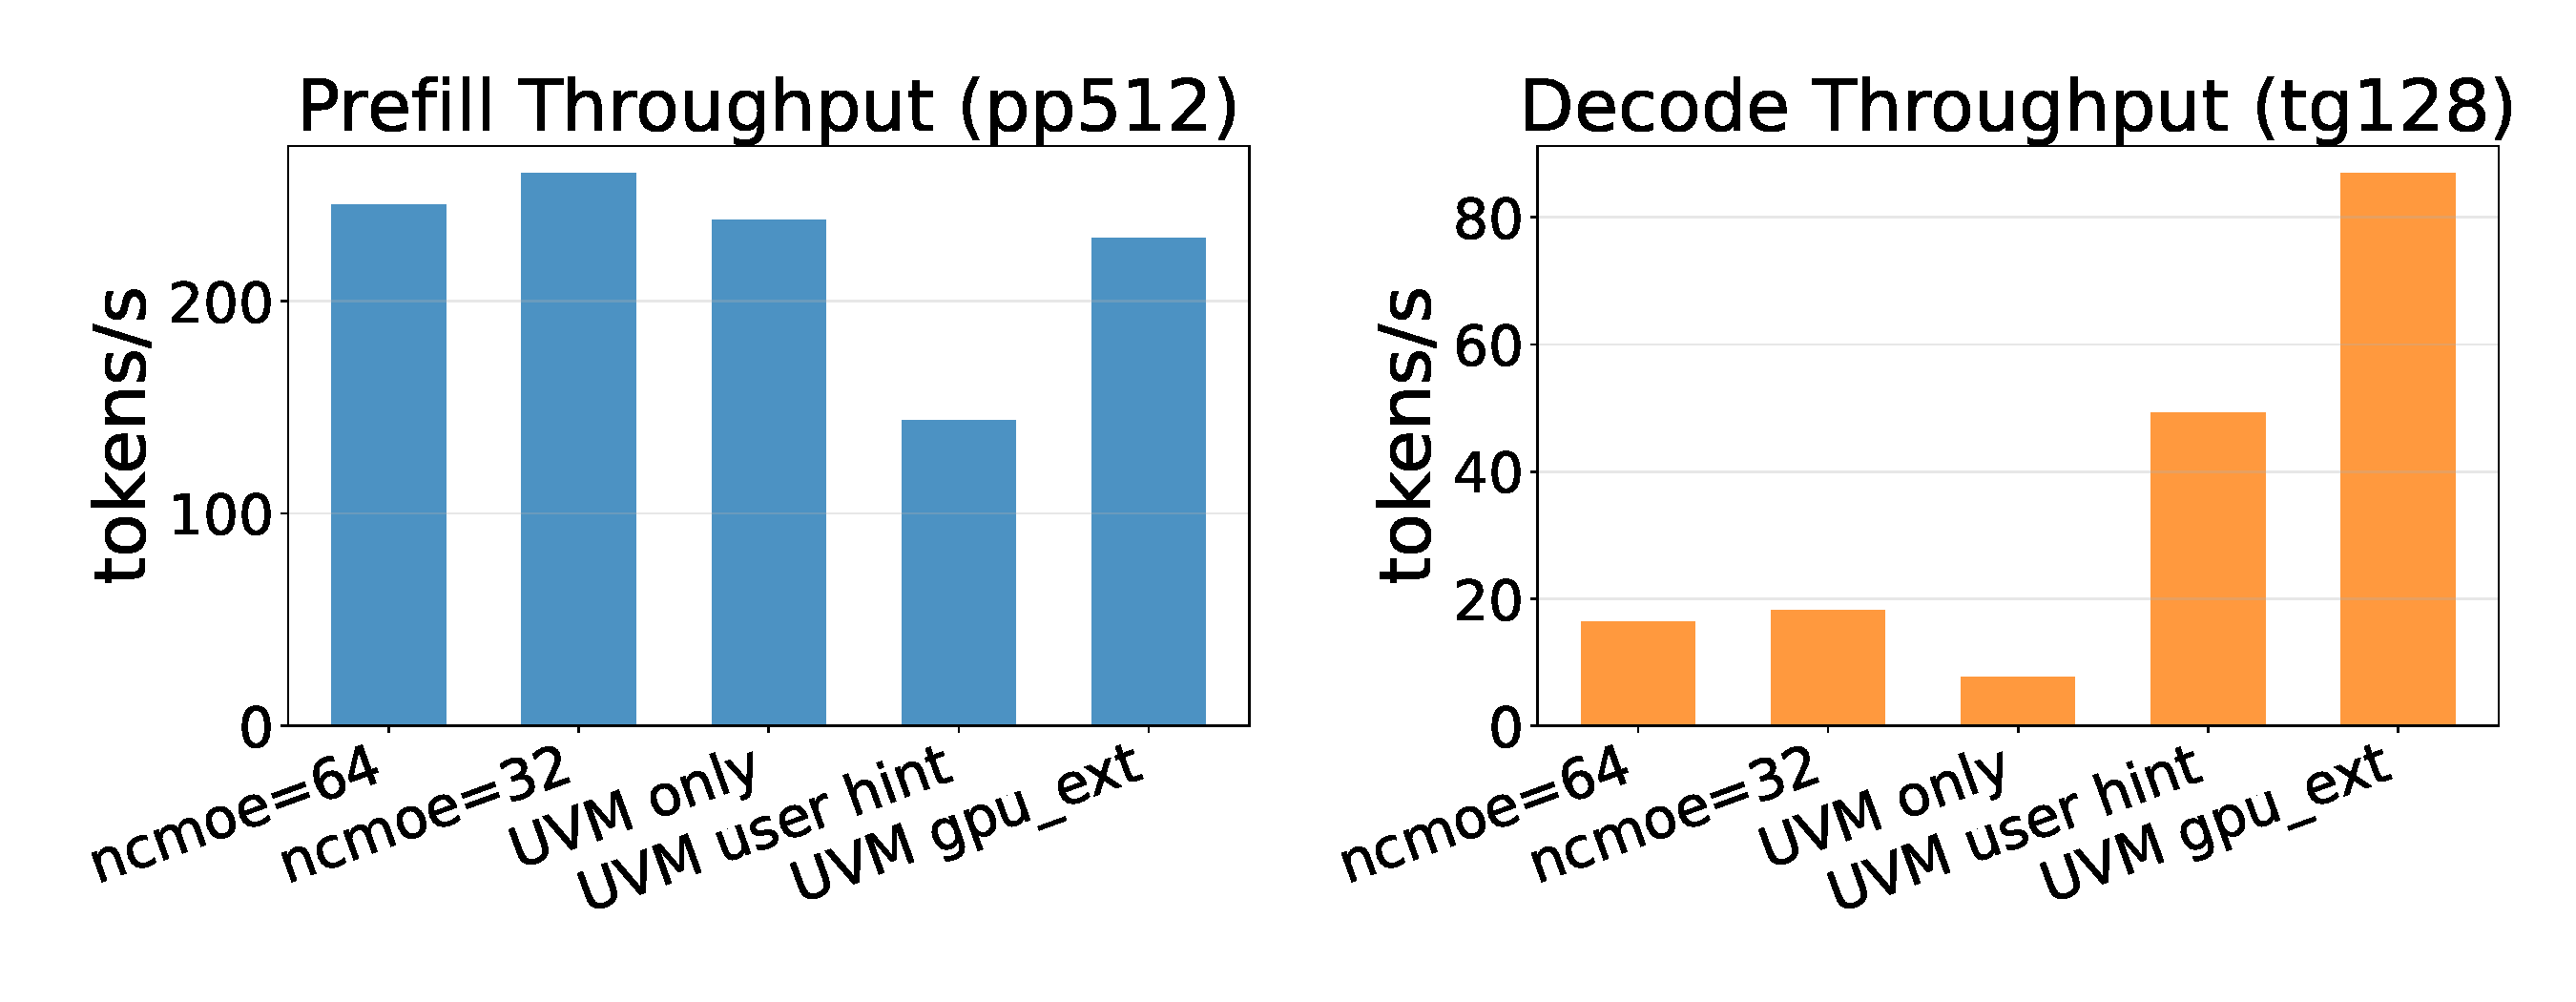
\includegraphics[width=\columnwidth]{img/results-raw/llama.cpp/llama_uvm_combined_color.pdf}
\caption{Prefill (pp512) and decode (tg128) throughput for GPT-OSS-120B MoE (59~GiB) on RTX 5090 (32GB). \sys eBPF prefetching achieves \textbf{4.8$\times$ decode speedup} over llama.cpp's framework offloading (ncmoe=32), while maintaining competitive prefill performance (-12\%).}
\label{fig:llama-expert-offload}
\end{figure}

\paragraph{KV-cache Offloading (vLLM Qwen-30B MoE).}
We evaluate on the Qwen-30B FP8 MoE model ($\approx$30GB) on RTX 5090 (32GB). The model alone nearly fills GPU VRAM, so default no-offload configuration OOMs under load. We stress KV-cache growth by sending 100 concurrent requests from ShareGPT (single-round, no prefix caching), resulting in total memory footprint of 36--40GB (model + KV-cache for $\approx$60K tokens aggregate). Existing solutions typically offload either KV-cache or MoE experts, but not both; in contrast, UVM attempts on-demand migration of both, leading to thrashing.

We compare vLLM's CPU-offload mode (\texttt{--cpu-offload-gb 8}) against \sys with UVM and a simple sequential prefetch policy based on PCIe traffic patterns. This policy performs more aggressive prefetching than fixed heuristics, reducing thrashing and page faults. \sys improves mean and p99 time-to-first-token by 1.7--2$\times$ and decoding throughput by about 1.3$\times$ over vLLM's framework-managed offload (\Cref{fig:vllm-kv-offload}). Simply enabling UVM without \sys policies performs worse than vLLM's own offload; the \sys configuration is roughly 2--3$\times$ faster than this UVM-only baseline. This demonstrates that \sys's programmable driver-level policies can match or exceed SOTA framework-managed offloading while providing better p99 latency, even in single-tenant scenarios.

\begin{figure}
\centering
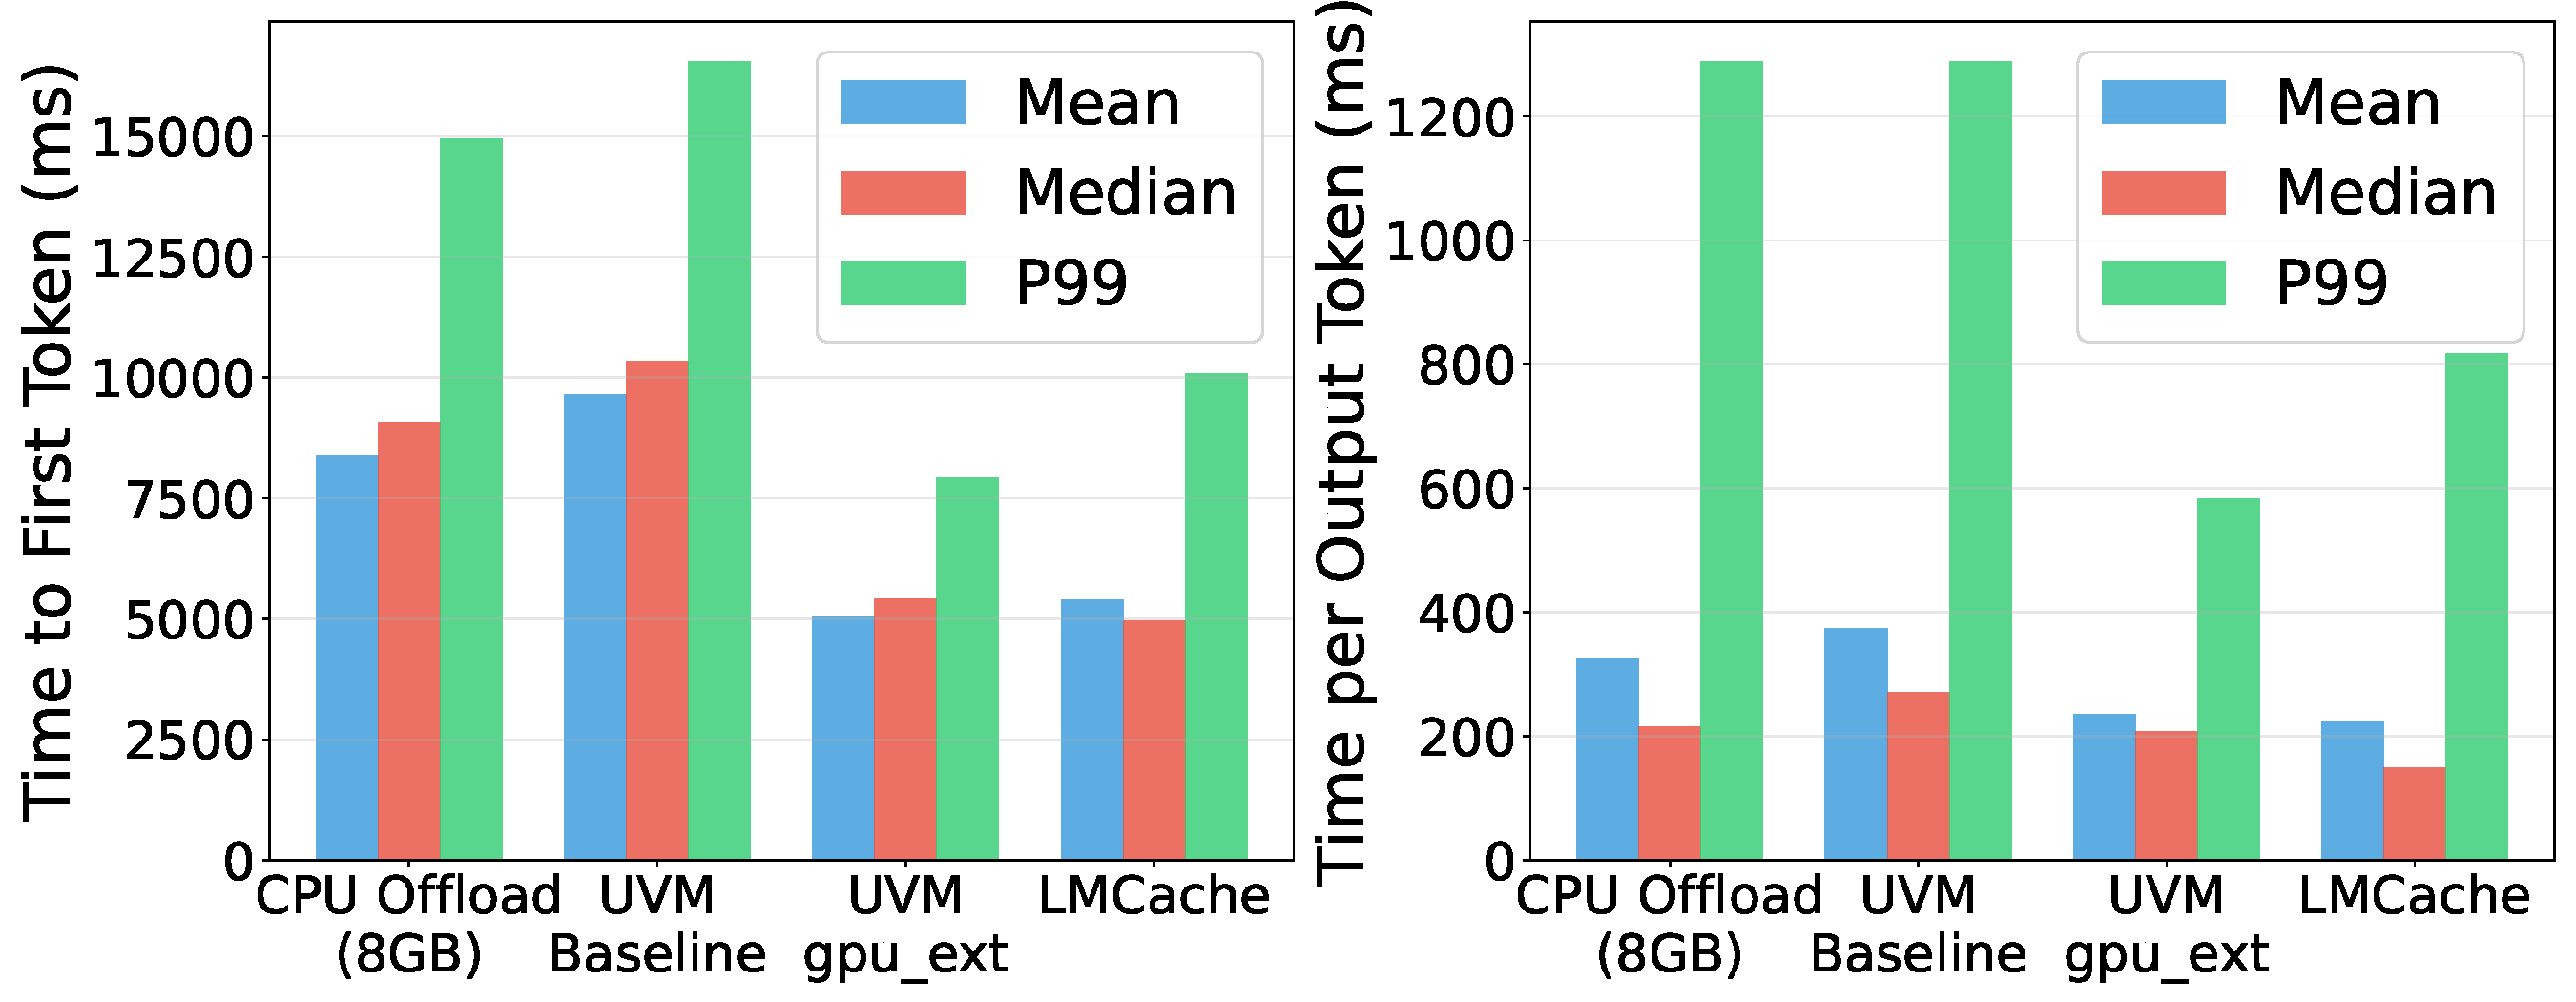
\includegraphics[width=\columnwidth]{img/results-raw/vllm/ttft_tpot_combined.pdf}
\caption{Time-to-first-token and decoding throughput for \sys KV-aware sequential prefetch policy vs vLLM CPU-offload on Qwen-30B FP8 MoE with 100 concurrent requests ($\approx$60K tokens KV-cache).}
\label{fig:vllm-kv-offload}
\end{figure}

\paragraph{Graph Neural Networks (GNN Training).}
We evaluate \sys on PyTorch-based GCN training with random graphs of varying sizes (1M--15M nodes, 10 edges/node). \Cref{fig:gnn-epoch} shows epoch time across five configurations: native GPU allocation (no UVM), UVM with and without user-space prefetching (\texttt{cudaMemPrefetchAsync}), and each UVM configuration with \sys eBPF-based scheduling optimization.

The key findings demonstrate that prefetching and eBPF scheduling are \emph{complementary} optimizations targeting different bottlenecks:

\begin{itemize}[leftmargin=*]
  \item \textbf{Prefetching eliminates page faults:} At 10M nodes (1.43$\times$ oversubscription), UVM without prefetch takes 70.06~s/epoch due to lazy page migration. Adding \texttt{cudaMemPrefetchAsync} reduces this to 12.76~s (\textbf{5.5$\times$ speedup}) by proactively migrating pages before GPU access.
  \item \textbf{eBPF optimizes page fault handling:} When prefetching is disabled, \sys's eBPF scheduler prioritizes the driver's page fault handling threads, reducing epoch time from 70.06~s to 26.47~s (\textbf{2.65$\times$ speedup}). This optimization is orthogonal to prefetching---when data fits in GPU memory with prefetch enabled, eBPF provides no additional benefit (12.76~s vs 12.17~s).
  \item \textbf{Severe oversubscription benefits from both:} At 15M nodes (2.17$\times$ oversubscription), runtime page faults occur even with prefetching. Here, \sys reduces epoch time from 215.82~s to 150.11~s (\textbf{1.44$\times$ speedup}), demonstrating that eBPF scheduling remains effective when memory pressure causes evictions during execution.
\end{itemize}

Native GPU allocation (no UVM) achieves the best performance when data fits in memory (1.89~s at 5M nodes) but fails with OOM beyond $\sim$8M nodes. UVM with \sys prefetching enables training at 15M nodes (2.17$\times$ oversubscription) with acceptable overhead. The CPU-side framework overhead for these policies is around 1\%, and device-side instrumentation adds 2--3\%.

\begin{figure}
\centering
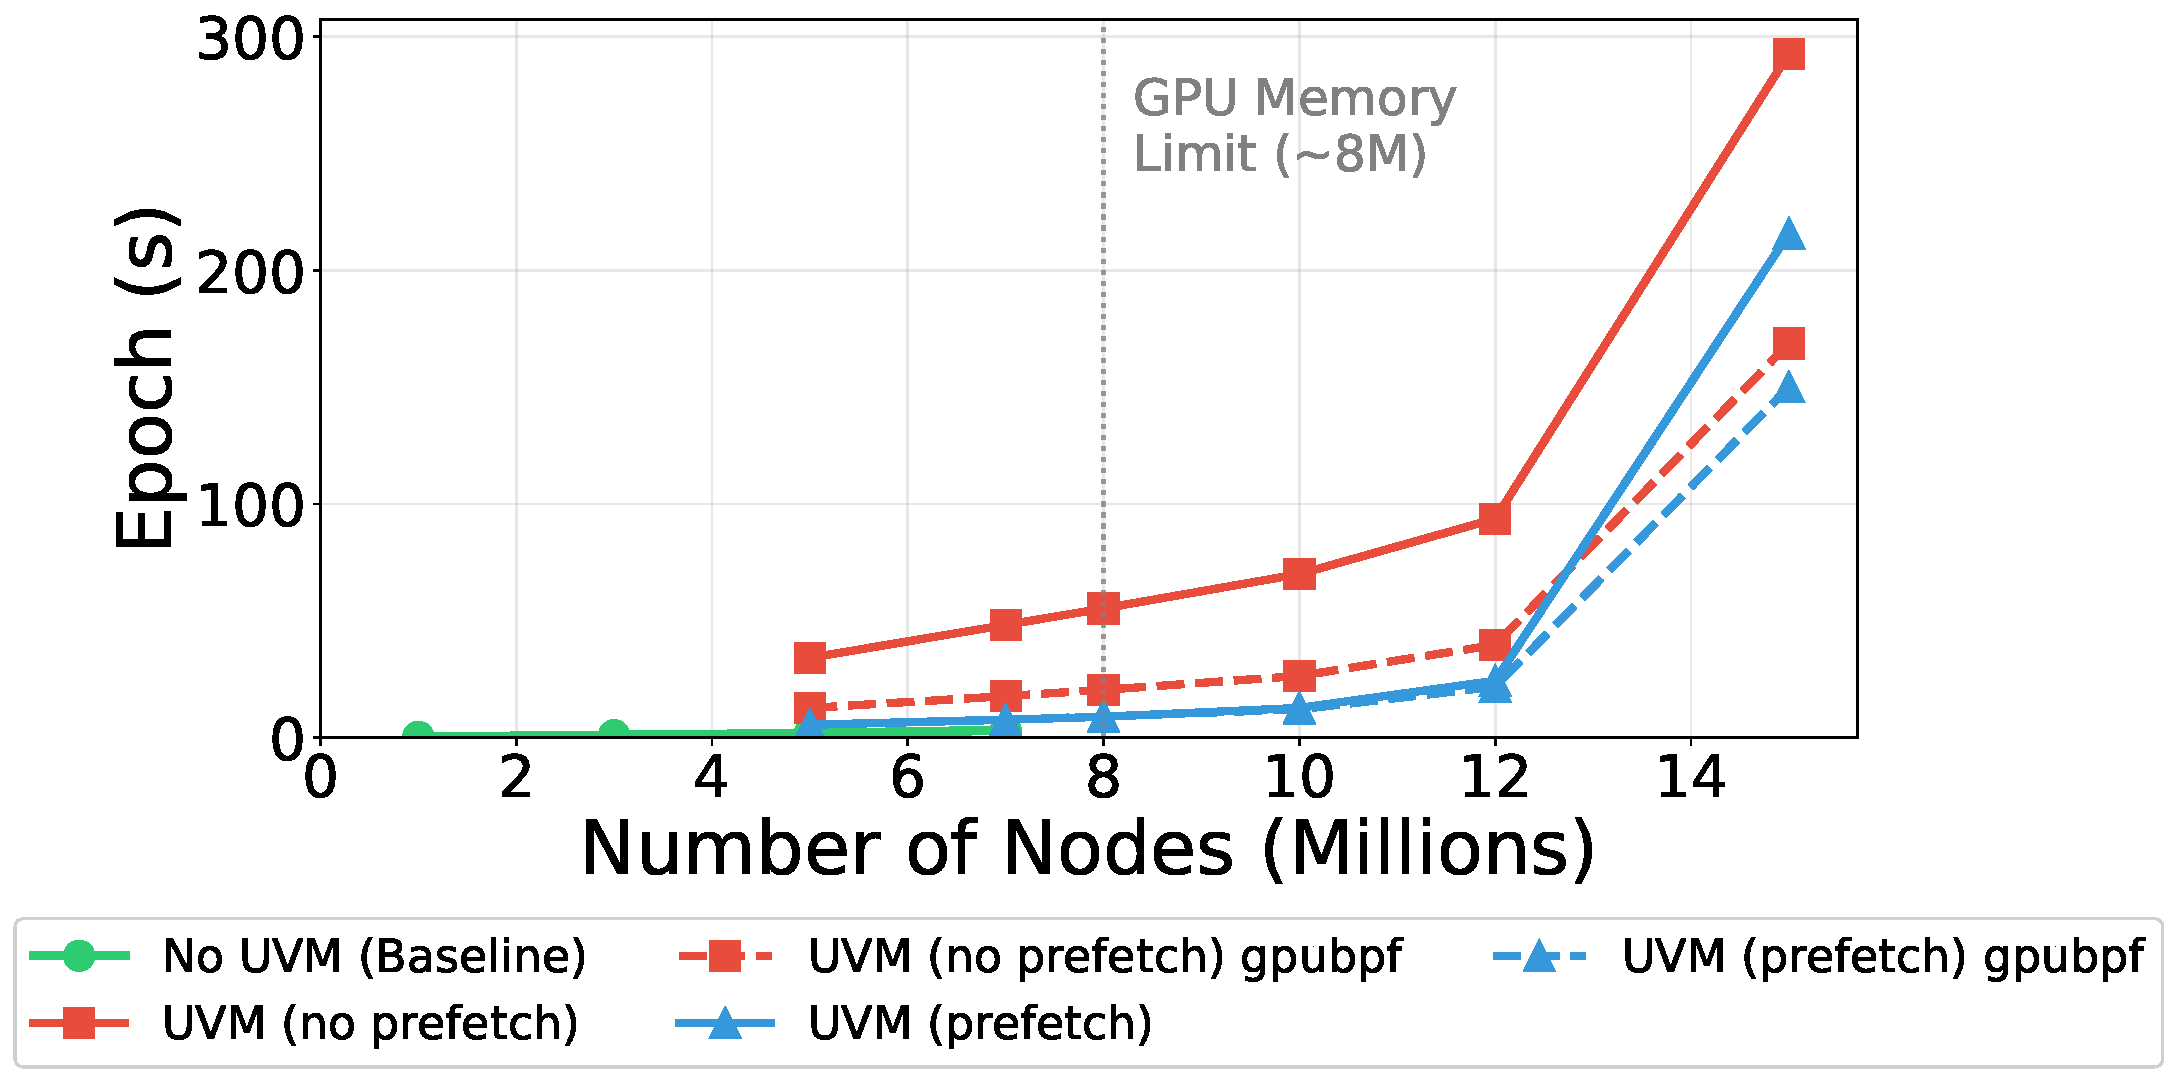
\includegraphics[width=\columnwidth]{img/results-raw/pytorch/uvm_benchmark_comparison.pdf}
\caption{GCN training epoch time vs graph size. Native GPU allocation (green) OOMs at $\sim$8M nodes. UVM without prefetch (red) suffers 30$\times$ overhead from page faults; \sys eBPF scheduling (dashed red) provides 2.65$\times$ speedup. UVM with prefetch (blue) achieves 5.5$\times$ speedup; at severe oversubscription (15M nodes), \sys (dashed blue) provides additional 1.44$\times$ improvement.}
\label{fig:gnn-epoch}
\end{figure}

\paragraph{Faiss Vector Search.}
We evaluate \sys on vector similarity search using the SIFT dataset with an IVF4096,Flat index. We scale the dataset from 20M (9.5GB, fits in memory) to 50M (24GB, near boundary) and 100M (48GB, exceeds 32GB GPU memory).
First, we establish the baseline: for the 20M dataset, GPU execution is 21$\times$ faster for index construction and roughly 29$\times$ faster for search compared to CPU, confirming the critical value of GPU acceleration.
For the larger datasets relying on UVM, we apply a \sys policy implementing adaptive tree-based prefetching.
For index construction, \sys reduces build time by 21.4\% on SIFT50M (16.77s $\to$ 13.19s) and 28.9\% on SIFT100M (67.77s $\to$ 48.15s). Notably, the benefits scale with dataset size, with build throughput improvement increasing from 27\% to 40\% as memory pressure grows.
For search workloads on the oversubscribed SIFT100M dataset, \sys reduces latency by 10--16\% across \texttt{nprobe} settings: 15.9\% improvement at nprobe=1 (14.04s $\to$ 11.80s) and 10.5\% at nprobe=16 (57.44s $\to$ 51.42s). The policy effectively hides latency by proactively fetching posting lists, increasing QPS by 11.7\% at nprobe=16 despite the random access patterns inherent in ANN search.

\begin{figure}
\centering
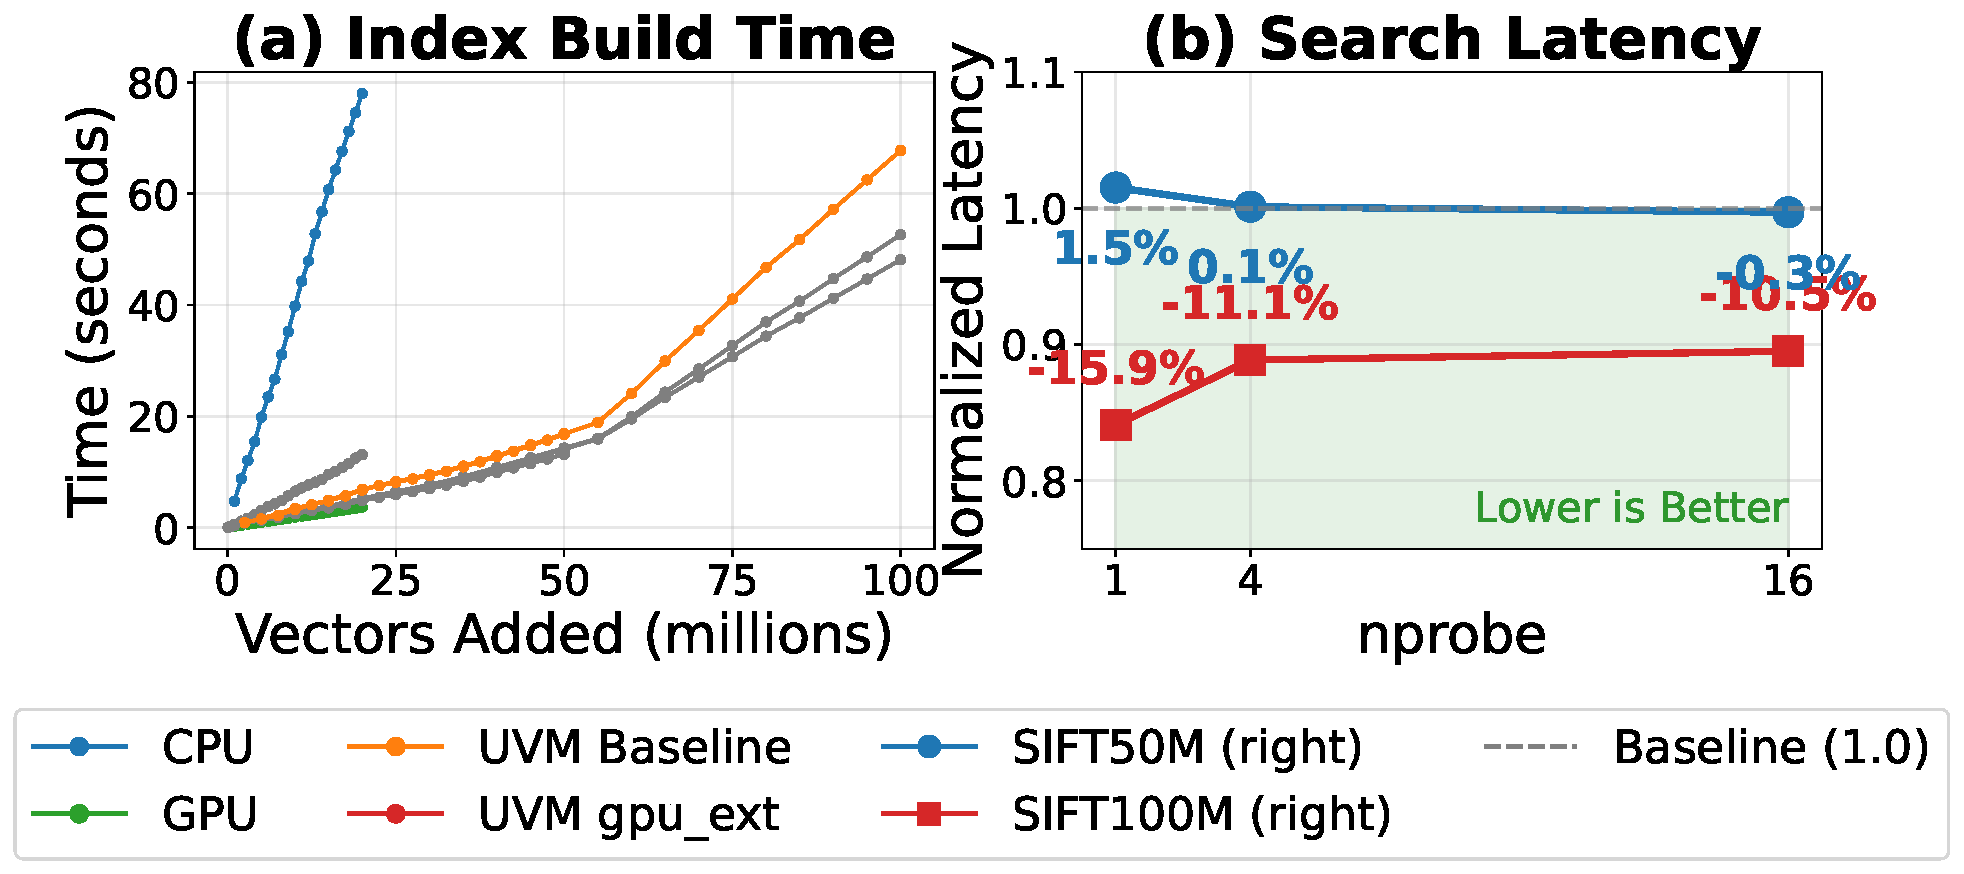
\includegraphics[width=\columnwidth]{img/results-raw/faiss/faiss_benchmark_results.pdf}
\caption{Faiss index build time and query throughput with \sys adaptive prefetch policy vs default UVM under oversubscribed index segments ($\approx$1.5$\times$ speedup).}
\label{fig:faiss-perf}
\end{figure}

Across these applications, the common pattern is that programmable region-based
placement and prefetch policies in \sys allow the system to exploit workload
structure (experts, KV-cache, graph structure, index layout) that existing UVM
policies and framework-level offload mechanisms cannot leverage without invasive
changes.

\subsection{RQ2: Multi-Tenant Memory, Bandwidth, and Scheduling}

We evaluate \sys's cross-layer policy framework on multi-tenant GPU workloads, comparing per-tenant policies against global policies and framework-managed approaches. We focus on tail latency, throughput, resource fairness, and GPU utilization.

\subsubsection{Microbenchmarks}

\paragraph{Multi-Tenant Timeslice Scheduler (LC + BE).}
We evaluate \sys's BPF struct\_ops scheduling policies on \emph{compute-bound} multi-tenant workloads where the bottleneck is GPU SM time rather than memory bandwidth. In this scenario, 2 latency-critical (LC) processes and 4 best-effort (BE) processes run concurrently, each with 4 CUDA streams submitting 50 compute kernels ($\sim$80ms/kernel). We compare the native scheduler against \sys with differentiated timeslices (LC: 1s, BE: 200$\mu$s), collecting 12,000 kernel launch latency samples over 10 rounds per configuration.

\Cref{fig:scheduler-latency} shows that \sys reduces the per-round P99 launch latency mean for LC workloads from 1188$\mu$s to 53$\mu$s (95.5\% reduction), while P99 standard deviation drops from 3405$\mu$s to 35$\mu$s (99\% reduction), demonstrating significantly improved scheduling stability. BE throughput remains essentially unchanged (+0.8\%), confirming that \sys's BPF struct\_ops can dramatically reduce LC tail latency without sacrificing BE throughput.

\begin{figure}
\centering
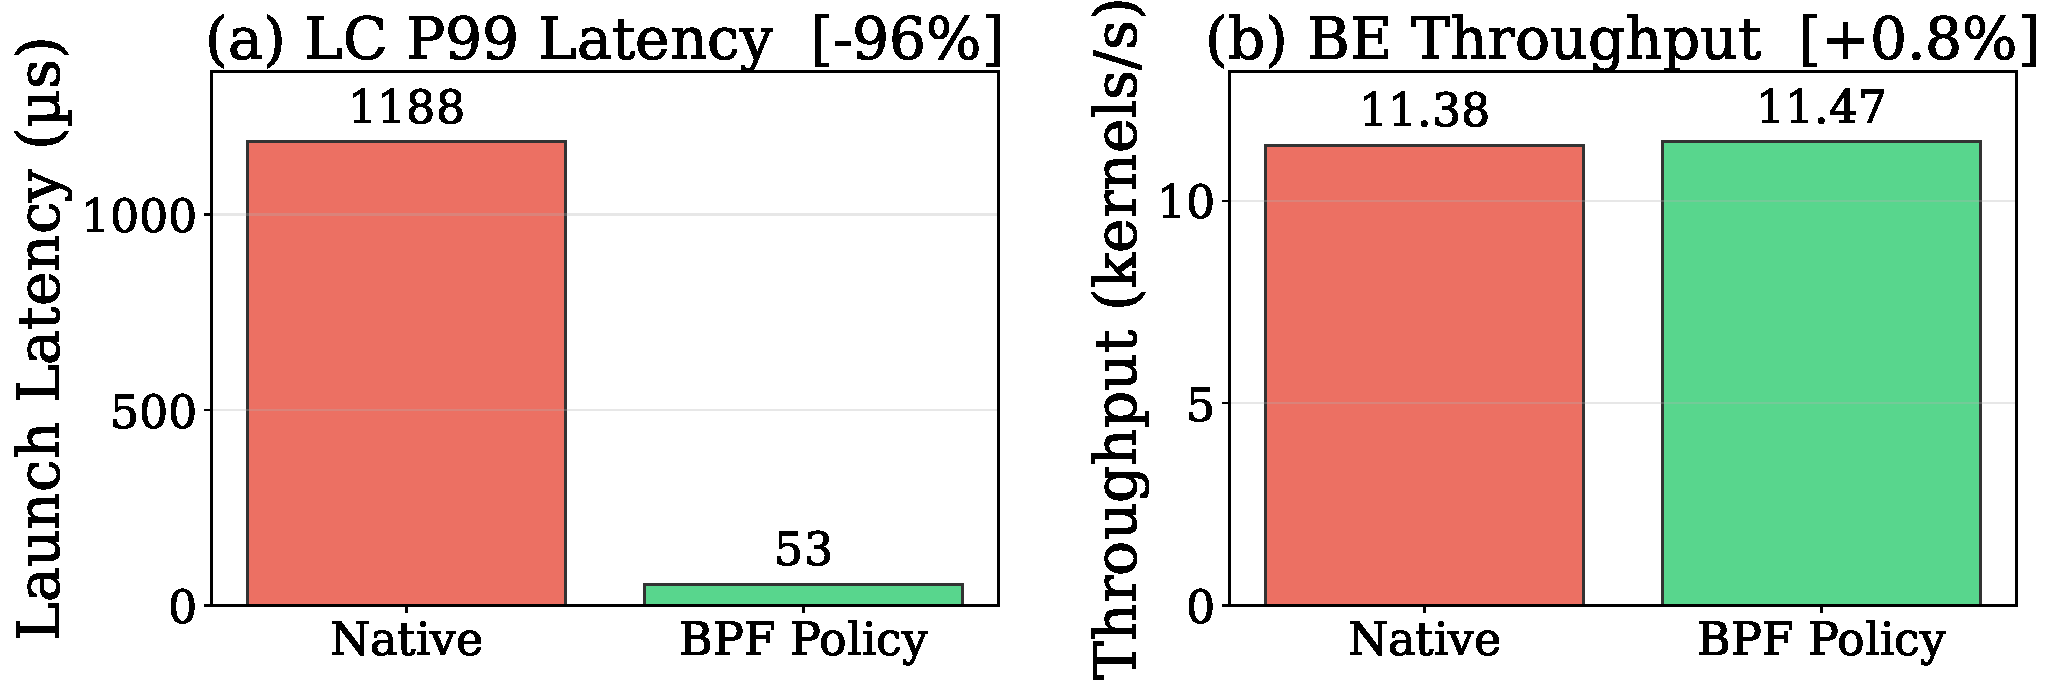
\includegraphics[width=\columnwidth]{img/results-raw/multi-tenant/scheduler_latency_throughput.pdf}
\caption{Multi-tenant GPU scheduling with \sys BPF struct\_ops policies on compute-bound workloads. LC P99 launch latency drops 95.5\% (1188$\mu$s $\rightarrow$ 53$\mu$s) with 99\% lower variance, while BE throughput remains unchanged (+0.8\%).}
\label{fig:scheduler-latency}
\end{figure}

\paragraph{Multi-Tenant Memory Priority Differentiation.}
We evaluate \sys's eBPF-based memory policies for priority differentiation on \emph{memory-bound} workloads under UVM oversubscription. We test three representative kernels: HotSpot (spatial locality), GEMM (compute-intensive), and K-Means (sparse access). Each experiment runs two concurrent processes competing for the same GPU memory, with \sys policies applying differentiated prefetch/eviction control based on process priority. We compare against: (1) no-policy multi-tenant execution, (2) single-process runtime (Single 1$\times$), and (3) the theoretical optimum for two workloads (2$\times$Single 1$\times$).

\Cref{fig:all-kernels-priority} shows that without policies, both processes degrade equally severely due to memory thrashing, with completion times 20--50$\times$ slower than single-process execution and less than 0.2\% difference between them. With \sys memory priority policies enabled, total completion time improves by 55--92\% compared to the no-policy baseline. High-priority processes complete 6--19\% faster than low-priority ones, demonstrating effective priority enforcement. In the best case, K-Means drops from 85.5s to 6.6s, approaching the theoretical lower bound of 2$\times$Single 1$\times$ (3.9s $\times$ 2 $\approx$ 7.8s). Prefetch and eviction policies show nearly identical effectiveness (<1\% difference), indicating that prefetch control is the dominant optimization in these workloads.

Crucially, scheduler timeslice policies are \emph{ineffective} for these memory-bound workloads (<1\% improvement), because the bottleneck is UVM page faults rather than GPU compute time. Memory policies directly control prefetch/eviction behavior, addressing the actual bottleneck. This demonstrates that \sys's layered policy framework allows operators to apply the right policy for each workload characteristic: scheduler policies for compute-bound scenarios, memory policies for memory-bound scenarios.

\begin{figure}
\centering
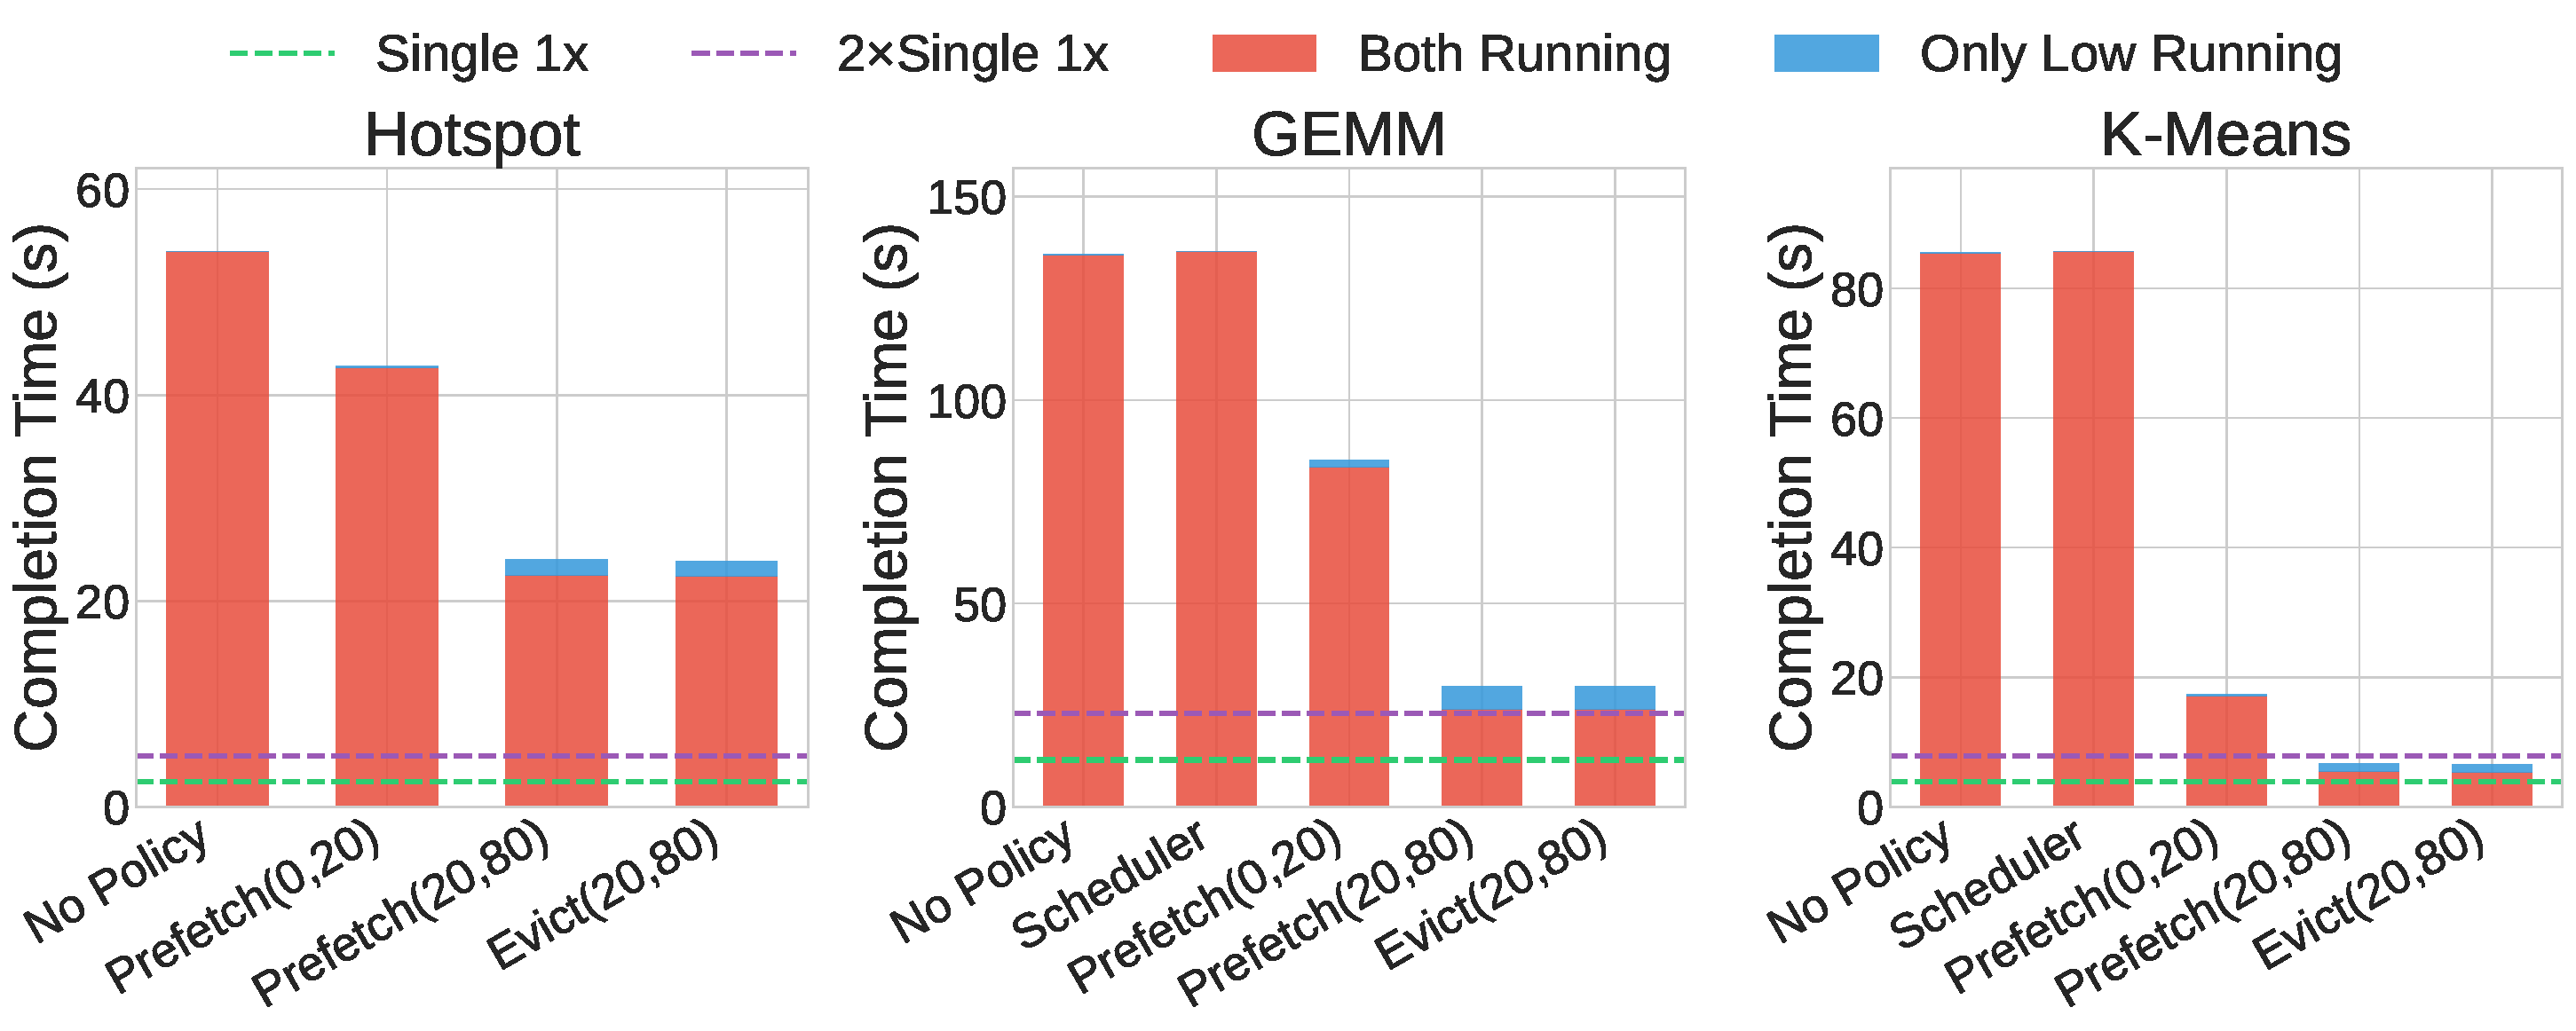
\includegraphics[width=\columnwidth]{img/results-raw/multi-tenant/all_kernels_stacked.pdf}
\caption{Multi-tenant memory priority differentiation on oversubscribed UVM workloads. \sys policies reduce total completion time by 55--92\% and enforce 6--19\% faster completion for high-priority tenants. Scheduler policies are ineffective (<1\%) on these memory-bound workloads. Single 1$\times$ shows ideal single-process time; 2$\times$Single 1$\times$ is the theoretical lower bound.}
\label{fig:all-kernels-priority}
\end{figure}

\subsubsection{Case Studies}

\paragraph{Two-Tenant: High-Priority LLM Inference + Background Training.}
We run two tenants sharing a single GPU: T1 is a high-priority \texttt{llama.cpp} inference service (LC workload) serving 100 ShareGPT prompts at 0.2 RPS, and T2 is a background PyTorch GNN training job (BE workload) with 8M nodes requiring 36GB peak memory (oversubscribed). We compare default UVM (driver FIFO/LRU) against \sys per-tenant memory policies where the LC tenant receives prefetch priority and the BE tenant yields bandwidth during inference.

\Cref{fig:two-tenant} shows the results. For the LC workload, \sys reduces mean TPOT by 45\% (19.7ms $\rightarrow$ 10.9ms) and P99 TPOT by 40\% (56.1ms $\rightarrow$ 33.4ms), bringing token generation latency from 5.4$\times$ single baseline down to 3.0$\times$. TTFT also improves by 20\% (428ms $\rightarrow$ 341ms mean) and 14\% at P99 (1392ms $\rightarrow$ 1203ms). Critically, \sys achieves a \emph{win-win}: GNN training simultaneously improves by 28\% (23.2s $\rightarrow$ 16.7s per epoch), approaching the ideal 2$\times$ single baseline (18.0s). This demonstrates that \sys's tenant-aware policies reduce memory contention for both workloads, rather than simply prioritizing one at the expense of the other.

\begin{figure}
\centering
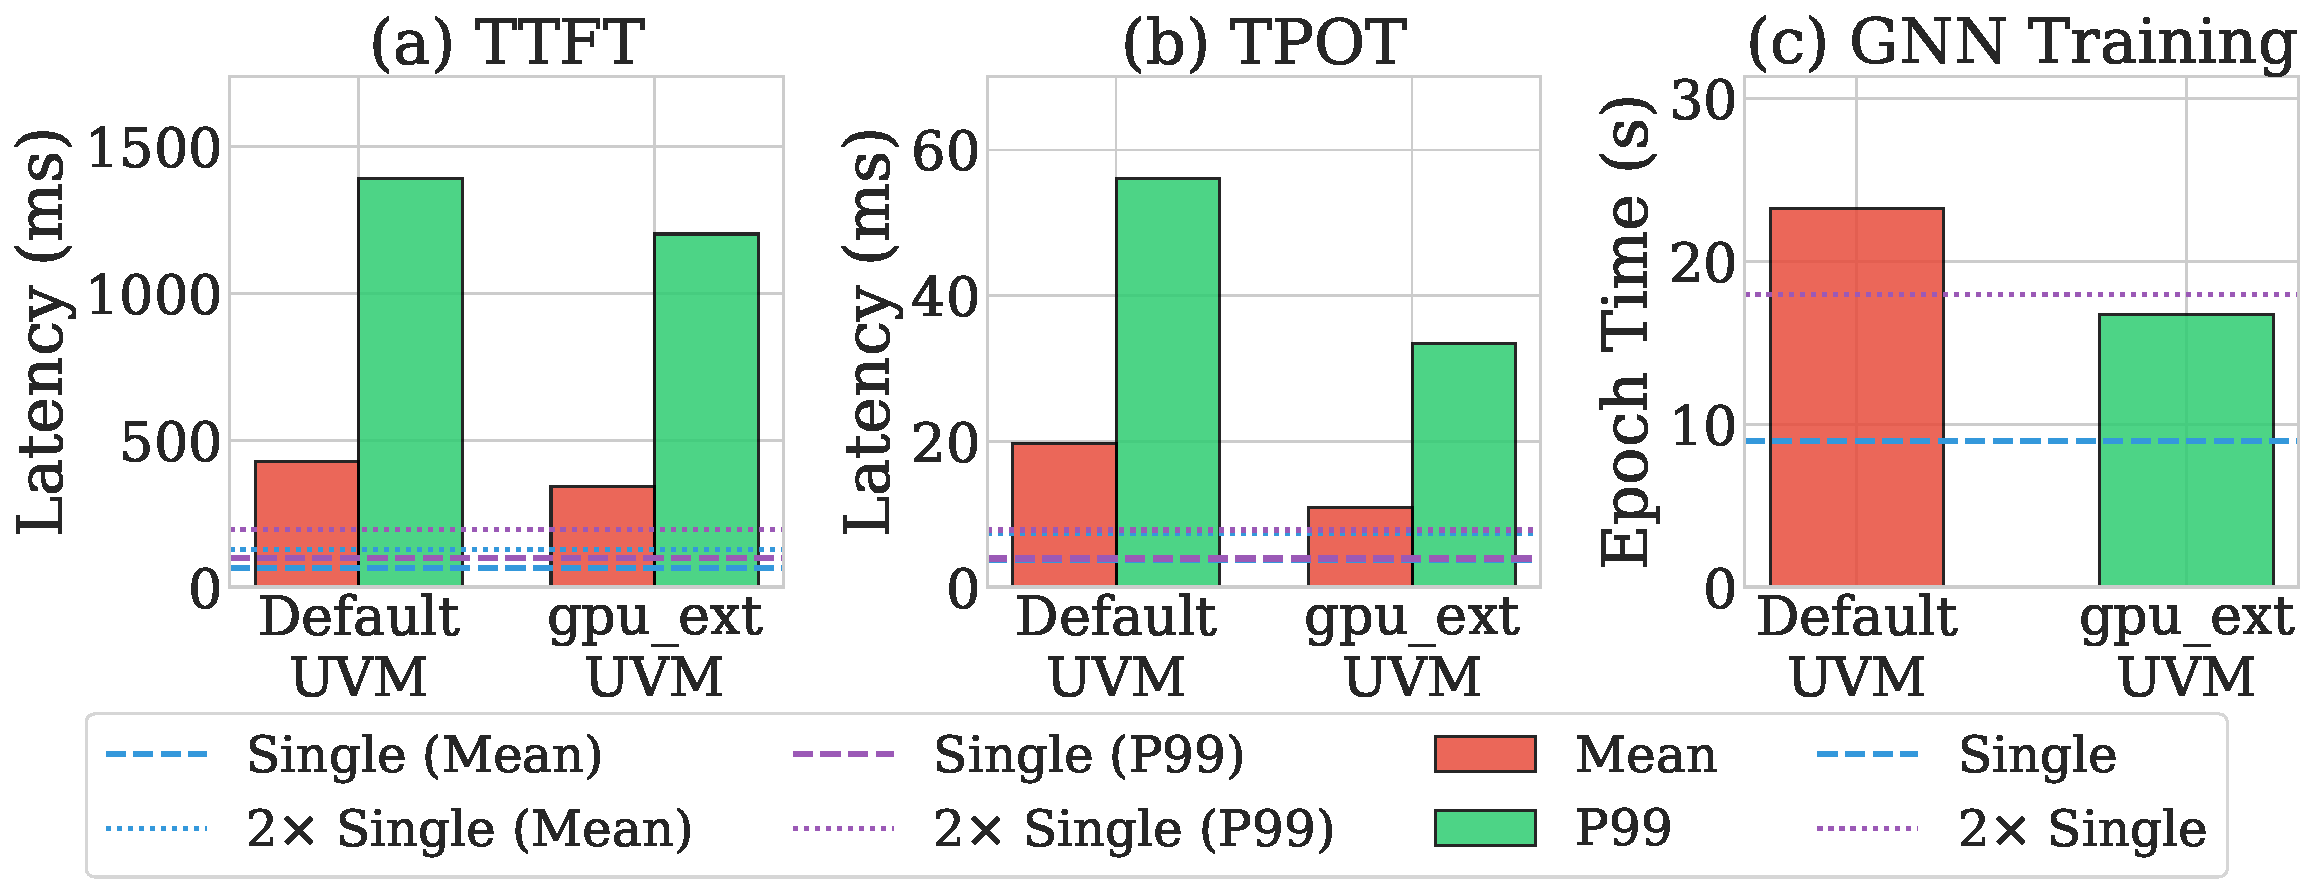
\includegraphics[width=\columnwidth]{img/results-raw/multi-tenant/fig_colocated_results.pdf}
\caption{Two-tenant co-location: \texttt{llama.cpp} inference (LC) + GNN training (BE). \sys reduces LC latency by 40--45\% while simultaneously improving BE training by 28\%. Dashed lines show single-tenant baselines; dotted lines show 2$\times$ single (ideal fair share).}
\label{fig:two-tenant}
\end{figure}

Overall, \sys's per-tenant policies provide clear tail-latency and fairness benefits in multi-tenant workloads, achieving significant improvements for high-priority tenants while also benefiting background jobs through reduced memory thrashing.

\subsection{RQ3: Programmability and Mechanism Overhead}

We evaluate \sys's programmability by examining policy complexity and reuse, and quantify the efficiency of its core mechanisms and observability capabilities.

\paragraph{Support Matrix.}
\Cref{tab:support-matrix} shows the policies implemented for each workload, along with lines of code (host eBPF + device eBPF) and measured overhead. All policies attach to unmodified frameworks via \sys's runtime instrumentation. The key takeaway is that a few hundred lines of policy code can implement sophisticated cross-layer resource management without application changes.

\begin{table}[t]
\centering
\small

\begin{tabularx}{\columnwidth}{@{} X l c c @{}}
\toprule
\textbf{Policy} & \textbf{Tag} & \textbf{Domain} & \textbf{LOC} \\
\midrule
Global FIFO Eviction & Memory (Eviction) & Host & 145 \\
Global LFU Eviction & Memory (Eviction) & Host & 304 \\
Multi-tenant Quota LRU & Memory (Multi-tenant) & Host & 472 \\
Adaptive Seq. Prefetch & Memory (Prefetch) & Host & 375 \\
Stride Prefetch & Memory (Prefetch) & Host & 472 \\
Stride Prefetch & Memory (Prefetch) & Device & 45 \\
Tree-based Prefetch & Memory (Multi-tenant) & Host & 454 \\
Dynamic Timeslice & Scheduling & Host & 408 \\
Preemption Control & Scheduling & Host & 925 \\
MaxSteals (CLC) & Scheduling (Block) & Device & 19 \\
SelectiveBlocks (CLC) & Scheduling (Block) & Device & 16 \\
\bottomrule
\end{tabularx}
\caption{Policy support matrix. Domain indicates where the policy executes: Host (driver eBPF), Device (GPU eBPF), or both.}
\label{tab:support-matrix}
\end{table}


\paragraph{Policy Reuse Across Workloads.}
The region cache policy skeleton used for llama.cpp expert offloading can be adapted to vLLM KV-cache management by changing only the region identification helpers and ID mappings. Similarly, the sequential prefetch policy applies to both GNN adjacency blocks and Faiss index segments with minimal modification (TODO: X lines changed out of Y total). This demonstrates \sys's support for portable, reusable policy components.

\subsubsection{Runtime and Shared State Overhead}

We first quantify the overhead of the \sys runtime itself, independent of any
specific policy logic. We use a load/store latency benchmark that issues controlled memory accesses from GPU kernels, instrumented with \sys and with NVBit gpumemtrace.

\Cref{fig:runtime-overhead} shows per-access latency slowdown under
\sys and NVBit as access sizes increase. \sys adds substantially less latency
than NVBit, remaining low and stable below 128~KB and increasing modestly
thereafter. Lightweight launch-time injection and warp-level execution of \sys handlers keep overhead low.

\begin{figure}
\centering
\fbox{\parbox{0.5\textwidth}{\centering [Figure: Runtime Overhead]}}
\caption{Runtime overhead of \sys vs NVBit across varying access sizes.}
\label{fig:runtime-overhead}
\end{figure}

\subsubsection{Low-overhead GPU Observability}

We evaluate the suite of bcc-style observability tools built on \sys, measuring
accuracy, overhead, and practical utility across diverse workloads.

\paragraph{Thread divergence and workload balance.}
\texttt{kernelretsnoop} attaches to kernel return paths and records per-thread
timestamps. Applied to a matrix multiply kernel with boundary checks, it shows
that threads handling edge cases (5\% of total) incur 600--850~ns longer
execution than interior threads, with timestamps within 10~ns of hardware
performance counters and 2.1\% overhead. Refactoring boundary handling based on
this insight improves overall kernel performance by 8\%. \texttt{threadhist}
reveals load imbalance in a particle simulation with 1M particles across 256
blocks: it identifies a bimodal distribution of iterations per thread;
rebalancing particles based on this information yields an 18\% throughput
improvement with 1.8\% tool overhead.

\paragraph{Launch latency and memory behavior.}
\texttt{launchlate} combines host and device hooks to measure kernel launch
latency. On a pipeline of 50 small kernels (each around 100~µs execution time),
default synchronous execution yields 150--550~µs launch latency per kernel, for
a total runtime of 32~ms. Switching to CUDA graphs, guided by
\texttt{launchlate}, reduces this to 7.2~ms, with less than 0.5\% overhead.
\texttt{mem\_trace} instruments sampled memory operations and recovers per-warp
bank conflict rates within 2\% of hardware counters, with under 3\% end-to-end
overhead across GEMM, SpMV and stencil kernels (\Cref{tab:obs-overhead}).

\begin{table}[t]
\centering
\small
\begin{tabularx}{\columnwidth}{@{} X l c c @{}}
\toprule
\textbf{Tool} & \textbf{LOC} & \textbf{Domain} & \textbf{Overhead} \\
\midrule
kernelretsnoop & 153 & Device & \\
launchlate & 347 & Host+Device & \\
mem\_trace & 110 & Device & \\
gpu\_sched\_trace & 586 & Host & \\
prefetch\_trace & 430 & Host & \\
eviction\_trace & 398 & Host & \\
\bottomrule
\end{tabularx}
\caption{\sys-based observability tools.}
\label{tab:obs-overhead}
\end{table}

\paragraph{Comparison to CUPTI and NVBit.}
\Cref{fig:obs-comparison} compares \sys-based tools against CUPTI and
NVBit for common profiling tasks. CUPTI-based profiling incurs 15--25\%
overhead and typically requires kernel restarts; NVBit adds 30--45\%
overhead for similar metrics. \sys tools average 2--3\% overhead and support
live instrumentation without interrupting execution.

\begin{figure}
\centering
\fbox{\parbox{\columnwidth}{\centering [Figure: Observability Tool Comparison]}}
\caption{Comparison of \sys observability tools vs CUPTI and NVBit across GEMM, SpMV, and stencil kernels. \sys achieves 2--3\% overhead vs CUPTI 15--25\% and NVBit 30--45\%.}
\label{fig:obs-comparison}
\end{figure}

\paragraph{Device-side Microbenchmarks and Optimization Effects.}
We evaluate device-side \sys mechanisms using a vector-add microbenchmark (32 elements, 10K iterations) on RTX 5090. \Cref{fig:microbench}(a) compares latency before and after our SIMT-aware warp-level execution optimizations (\S\ref{sec:verification}), with a baseline of 5.2~$\mu$s. Empty probe latency drops from 6.2~$\mu$s to 5.5~$\mu$s (-11\%), and exit probe from 6.2~$\mu$s to 5.3~$\mu$s (-14\%). More complex operations show larger improvements: array map lookup drops from 8.2~$\mu$s to 5.8~$\mu$s (-30\%), array map update from 11.1~$\mu$s to 7.0~$\mu$s (-37\%), and Memtrace from 9.4~$\mu$s to 6.1~$\mu$s (-35\%). \Cref{fig:microbench}(b) shows CPU map access via PCIe incurs ~33,700~$\mu$s latency---approximately 6000$\times$ slower than GPU-side operations, motivating \sys's hierarchical map design that keeps hot state on GPU.

\begin{figure*}
\centering
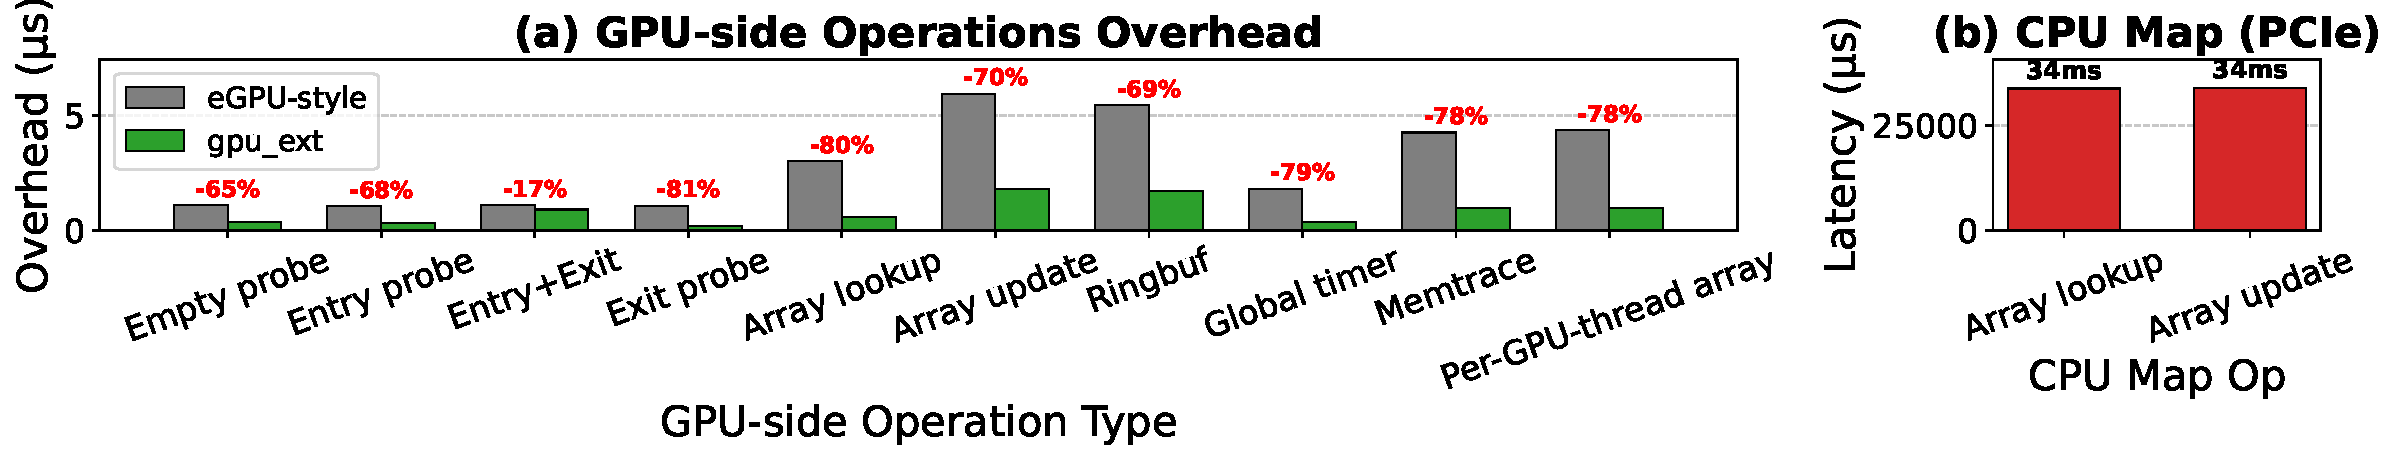
\includegraphics[width=\textwidth]{img/results-raw/runtime/microbench_comparison.pdf}
\caption{Device-side microbenchmark latency. (a) GPU-side operations before/after SIMT-aware optimizations show 11--37\% latency reduction. (b) CPU map access via PCIe is ~6000$\times$ slower than GPU-side operations.}
\label{fig:microbench}
\end{figure*}
